\documentclass[a4paper]{article} 
\addtolength{\hoffset}{-2.25cm}
\addtolength{\textwidth}{4.5cm}
\addtolength{\voffset}{-3.25cm}
\addtolength{\textheight}{5cm}
\setlength{\parskip}{0pt}
\setlength{\parindent}{0in}

\usepackage[square,sort,comma,numbers]{natbib}
\usepackage{blindtext} % Package to generate dummy text
\usepackage{charter} % Use the Charter font
\usepackage[utf8]{inputenc} % Use UTF-8 encoding
\usepackage{microtype} % Slightly tweak font spacing for aesthetics
\usepackage{amsthm, amsmath, amssymb} % Mathematical typesetting
\usepackage{float} % Improved interface for floating objects
\usepackage{hyperref} % For hyperlinks in the PDF
\usepackage{graphicx, multicol} % Enhanced support for graphics
\usepackage{xcolor} % Driver-independent color extensions
\usepackage{pseudocode} % Environment for specifying algorithms in a natural way
\usepackage[mmddyy]{datetime} % Uses YEAR-MONTH-DAY format for dates

\usepackage{fancyhdr} % Headers and footers
\pagestyle{fancy} % All pages have headers and footers
\fancyhead{}\renewcommand{\headrulewidth}{0pt} % Blank out the default header
\fancyfoot[L]{} % Custom footer text
\fancyfoot[C]{} % Custom footer text
\fancyfoot[R]{\thepage} % Custom footer text
\newcommand{\note}[1]{\marginpar{\scriptsize \textcolor{red}{#1}}} % Enables comments in red on margin

\DeclareMathOperator*{\argmin}{arg\,min}

%----------------------------------------------------------------------------------------


%-------------------------------
%	TITLE VARIABLES (identify your work!)
%-------------------------------

\newcommand{\yourname}{Balthazar Neveu | Jamy Lafenetre}
\newcommand{\youremail}{balthazarneveu@gmail.com | jamy.lafenetre@ens-paris-saclay.fr}
\newcommand{\assignmentnumber}{5}

\begin{document}

%-------------------------------
%	TITLE SECTION (do not modify unless you really need to)
%-------------------------------
\fancyhead[C]{}
\hrule \medskip
\begin{minipage}{0.295\textwidth} 
\raggedright
\footnotesize
\yourname \hfill\\
\youremail
\end{minipage}
\begin{minipage}{0.4\textwidth} 
\centering 
\large 
Lab session \# \assignmentnumber\\ 
\normalsize 
NPM 2024\\ 
\end{minipage}
\begin{minipage}{0.295\textwidth} 
\raggedleft
\today\hfill\\
\end{minipage}
\medskip\hrule 
\bigskip




%-------------------------------
%	ASSIGNMENT CONTENT (add your responses)
%-------------------------------


\section*{Question 1}
\begin{figure}[ht]
  \centering
  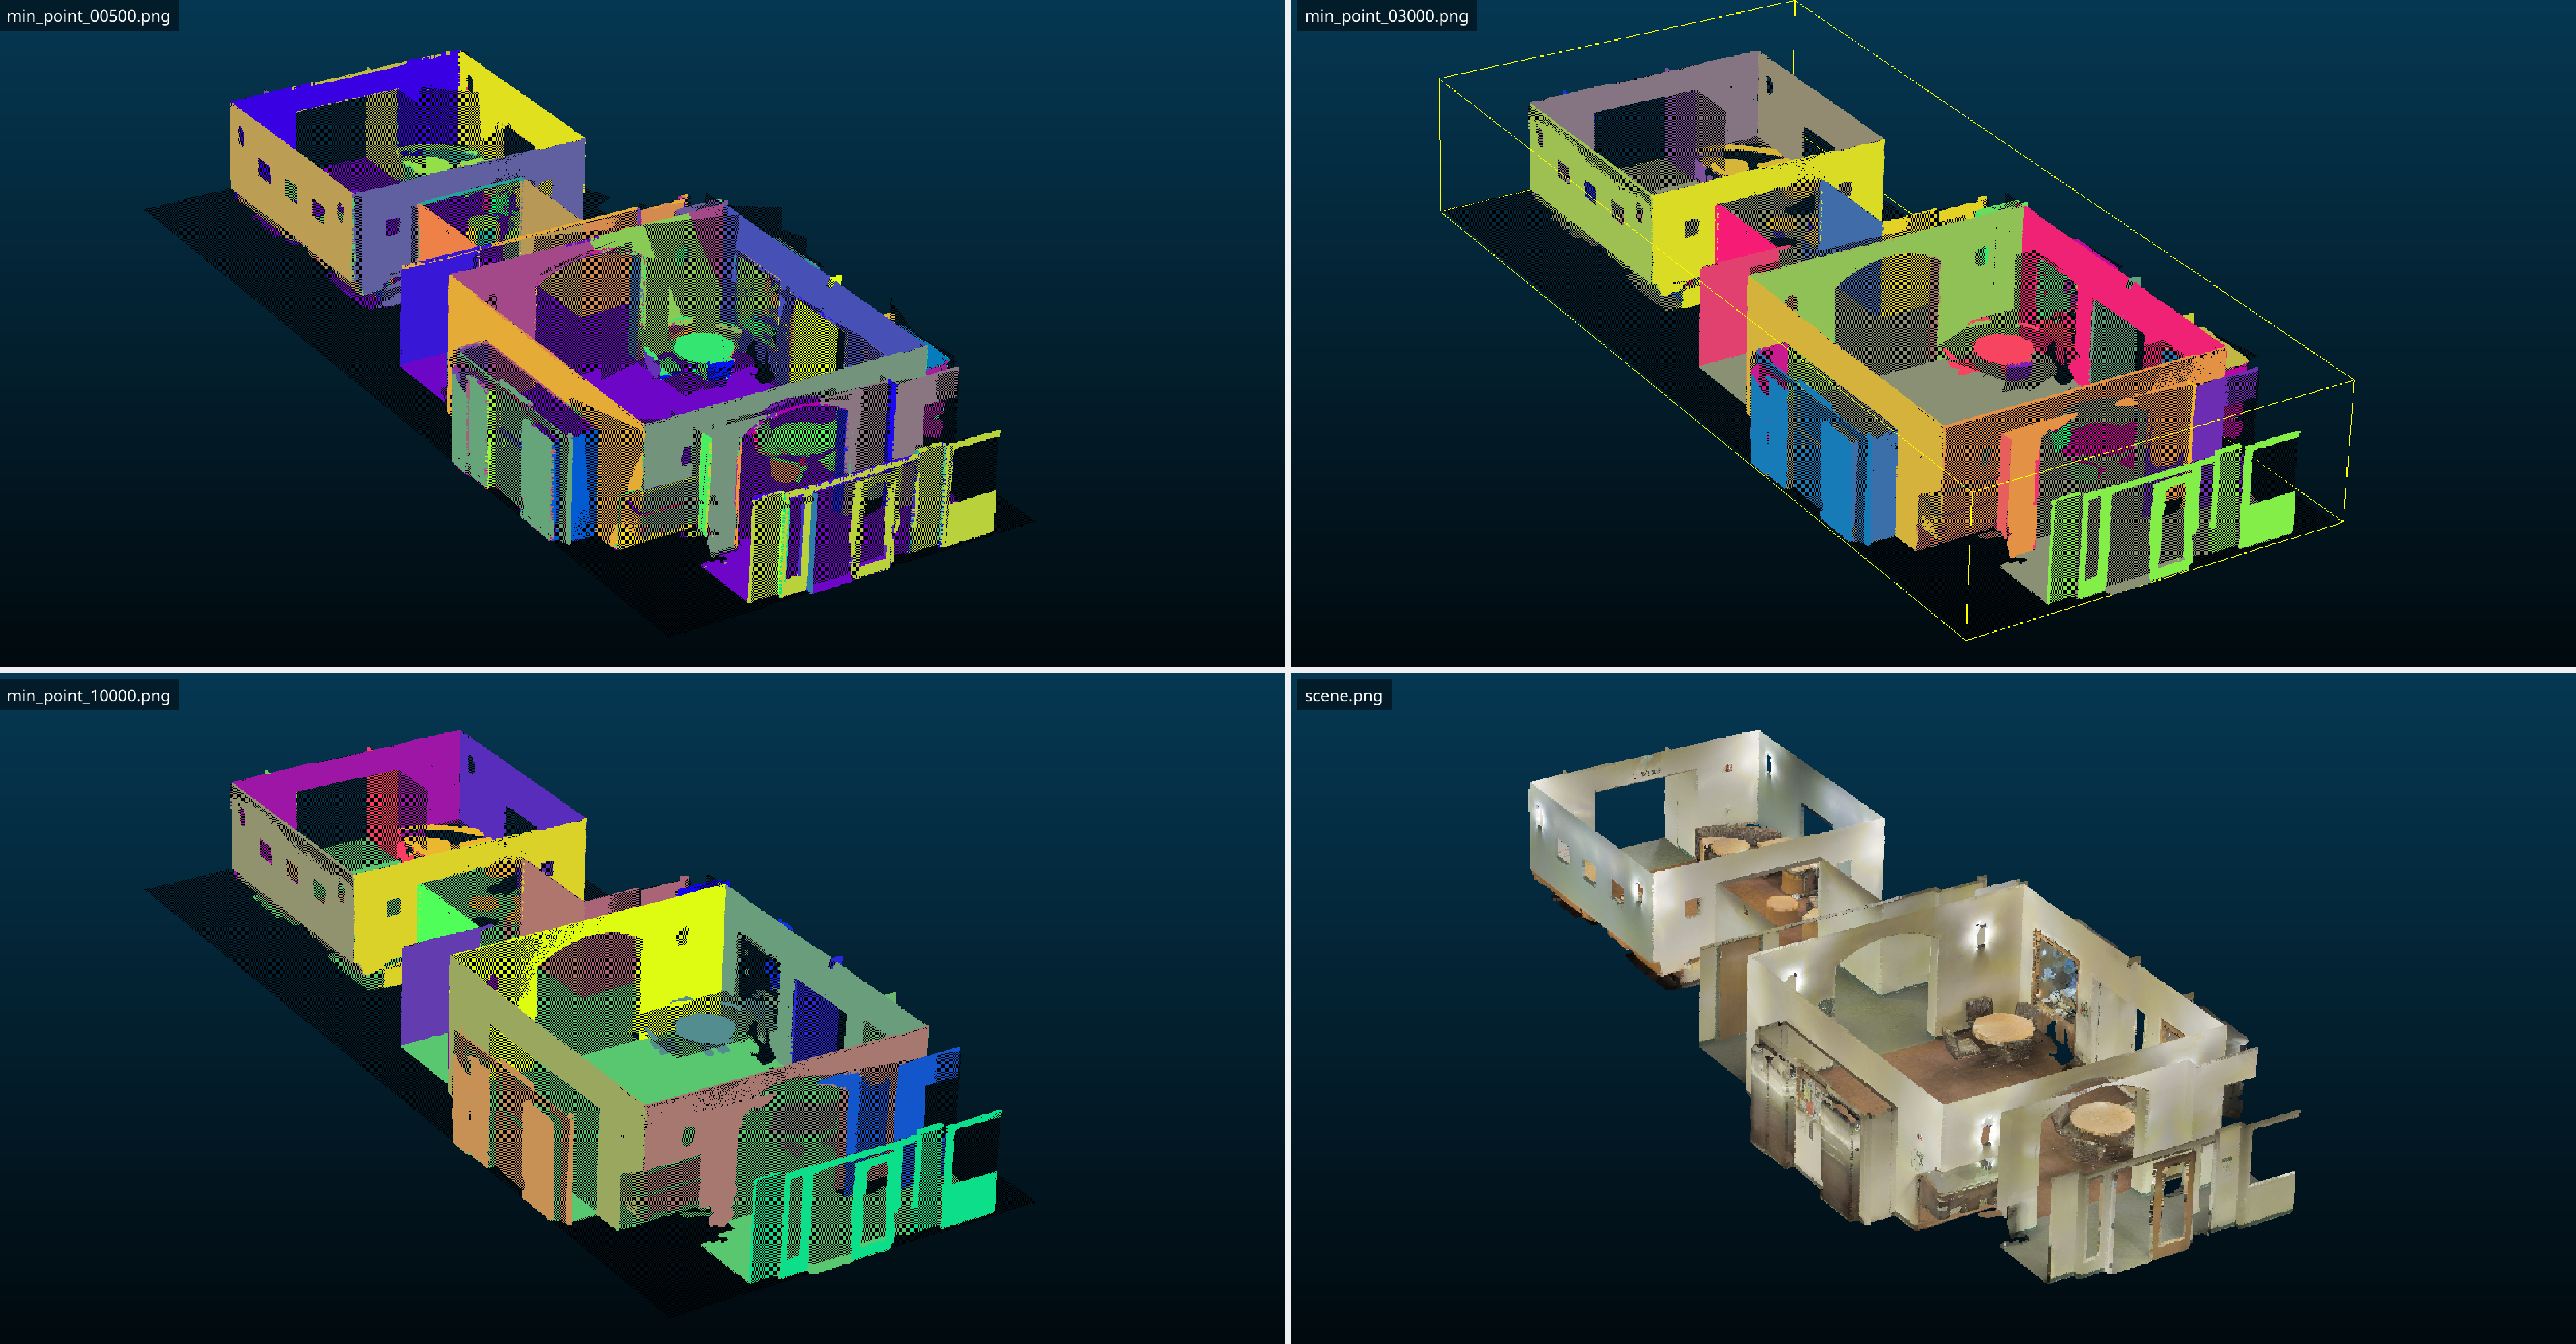
\includegraphics[width=0.9\linewidth]{figures/ransac_cloud_compare_comparison.png}
  \caption{RANSAC plane segmentation on the indoor point cloud.}
  \label{fig:ransac_overview}
\end{figure}



\section*{Implementation sanity check 1-2}
\begin{figure}[ht]
  \centering
  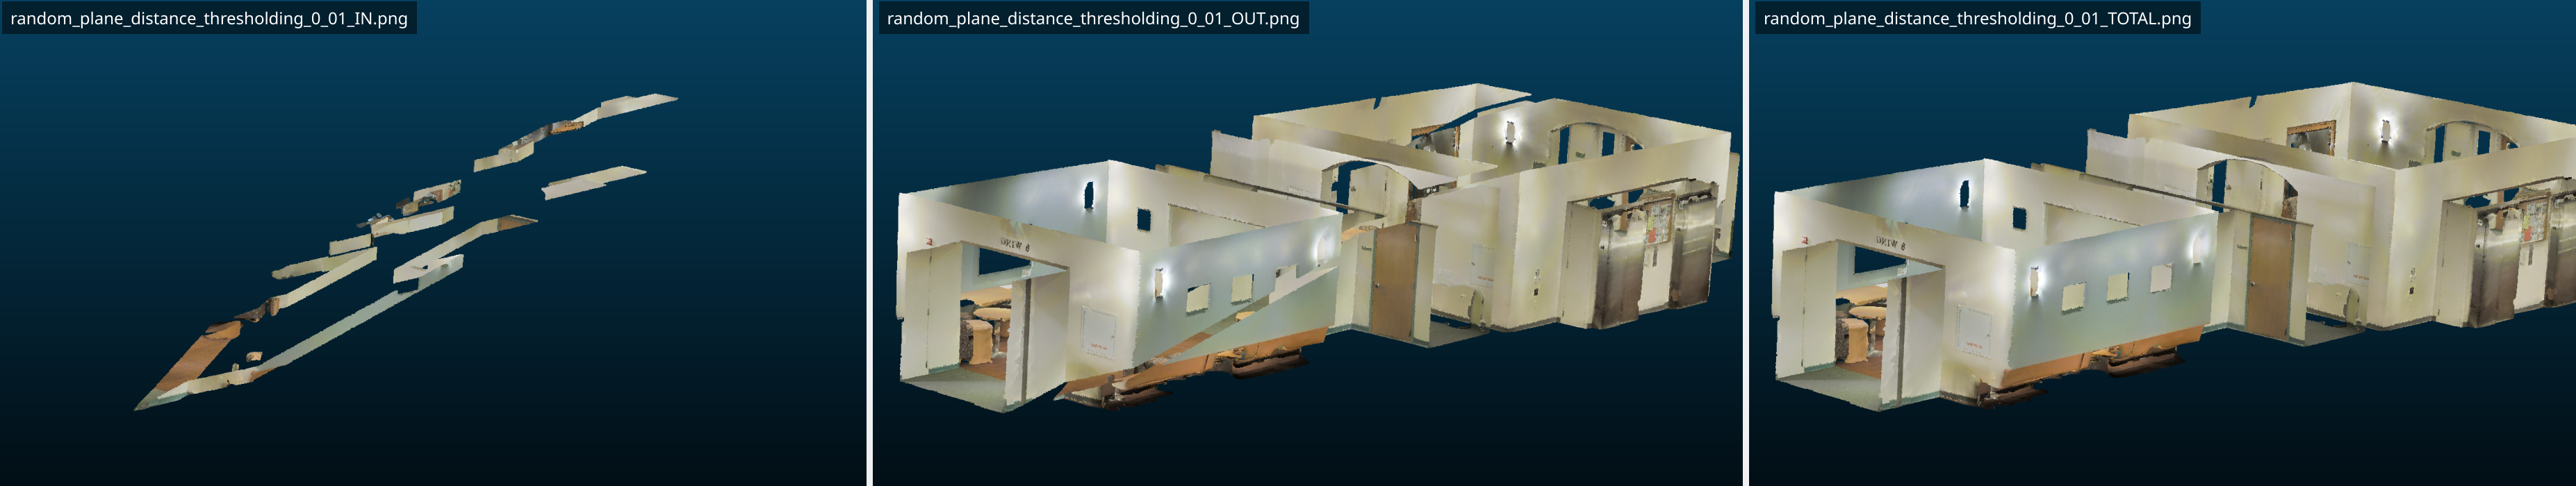
\includegraphics[width=0.9\linewidth]{figures/random_plane_distance_thresholding_0_01.png}
  \caption{Plane extraction from 3 points and thresholding. Left: Points close to the extracted planes. Middle: Points at a distance from the plane larger than the threshold. Right: original point cloud. }
  \label{fig:sanity_check_planes}
\end{figure}


\section*{Implementation sanity check 3}
RANSAC performed with pytorch in 0.34s on a very small laptop GPU Nvidia T500 with 4Gb of memory.
\begin{figure}[ht]
  \centering
  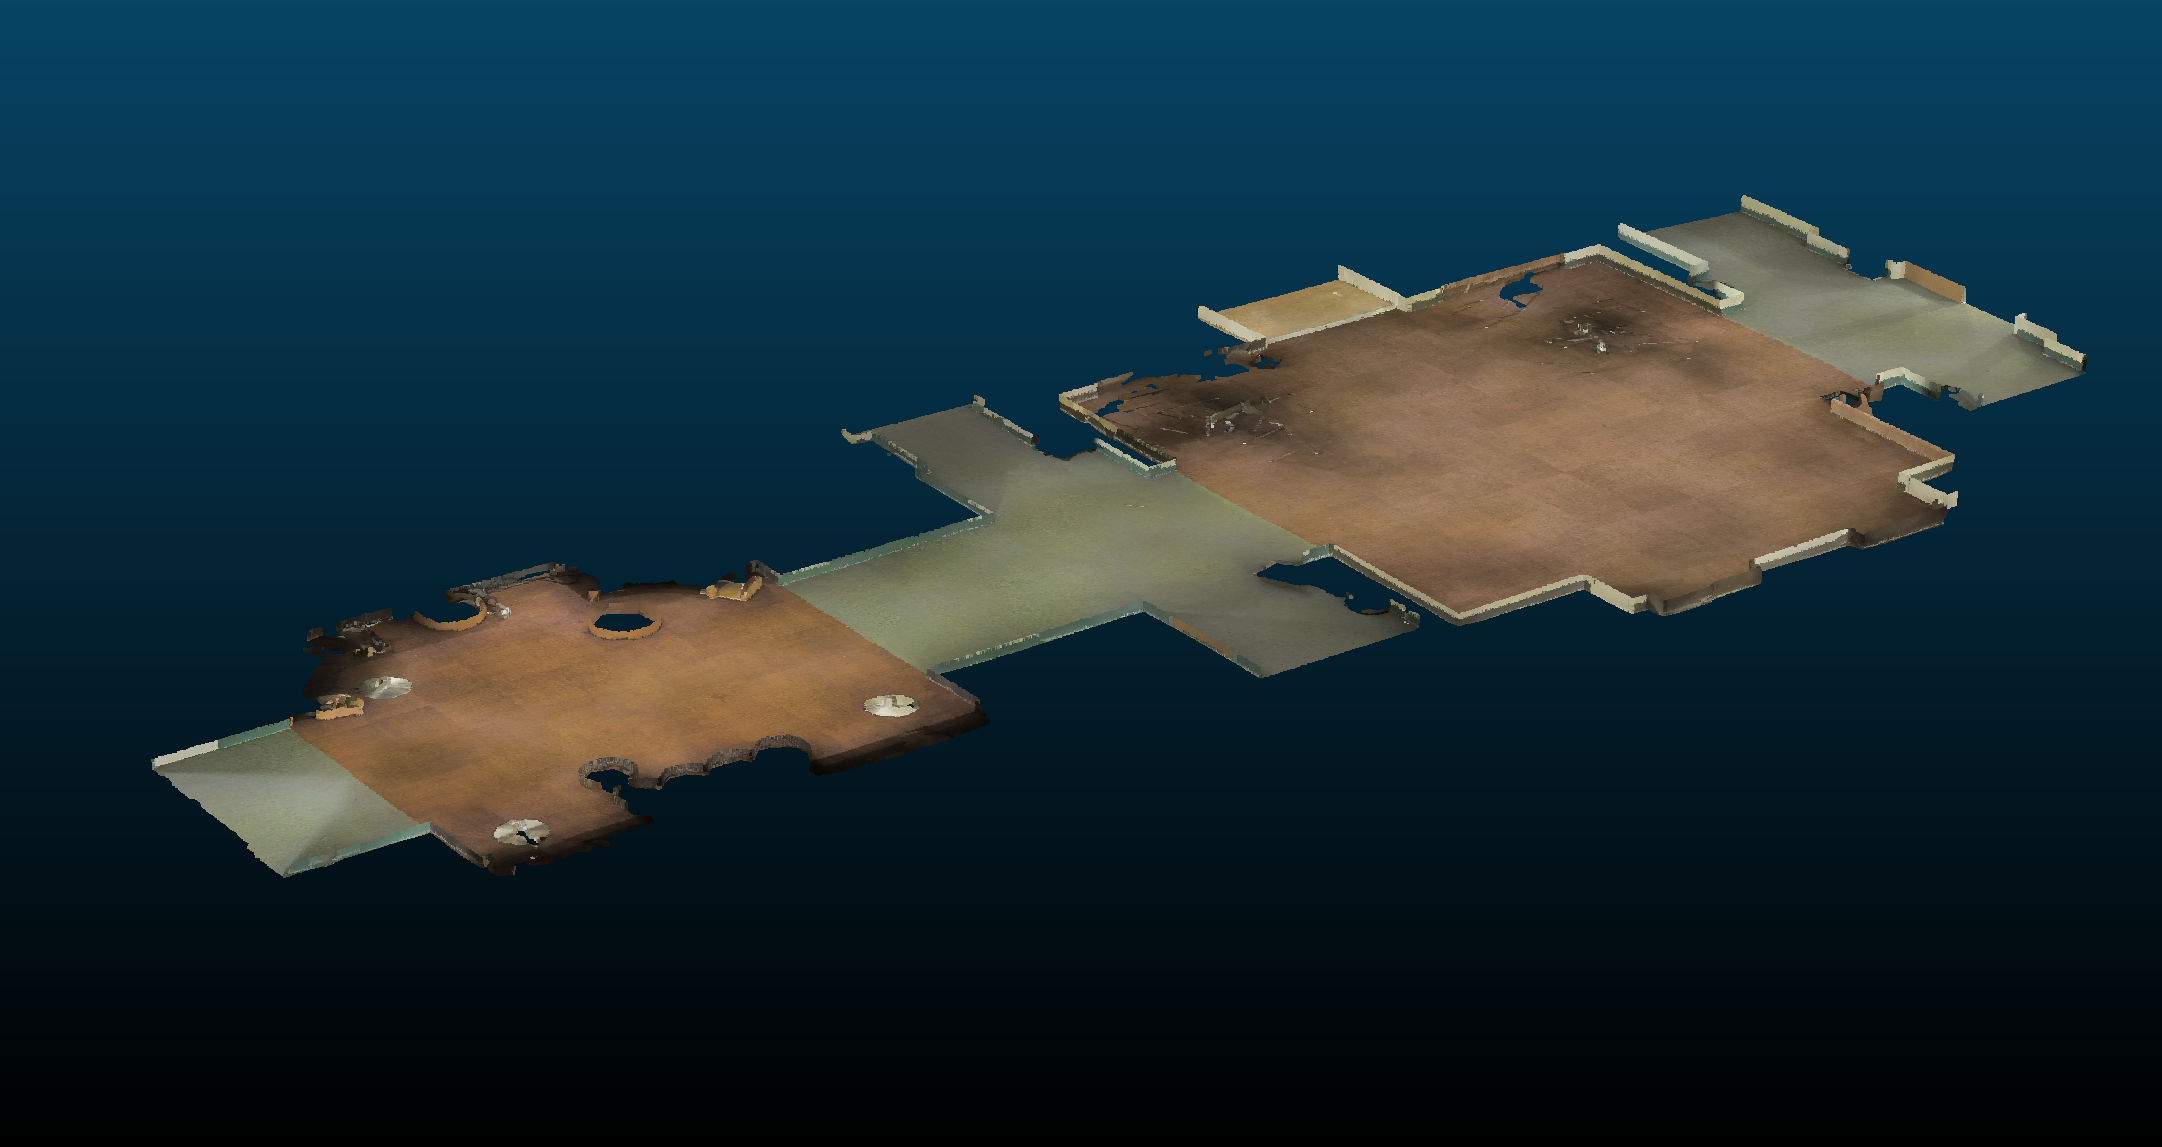
\includegraphics[width=0.3\linewidth]{figures/RANSAC_draw100_distance_thresholding_0_01_TOTAL.png}
  \caption{RANSAC Most important plane with 100 draws and thresholding 0.1. - Plane got 1051287 votes.}
  \label{fig:sanity_check_planes}
\end{figure}

\end{document}

